% Created 2020-08-31 Mon 15:53
% Intended LaTeX compiler: pdflatex
\documentclass[11pt]{article}
\usepackage[utf8]{inputenc}
\usepackage[T1]{fontenc}
\usepackage{graphicx}
\usepackage{grffile}
\usepackage{longtable}
\usepackage{wrapfig}
\usepackage{rotating}
\usepackage[normalem]{ulem}
\usepackage{amsmath}
\usepackage{textcomp}
\usepackage{amssymb}
\usepackage{capt-of}
\usepackage{hyperref}
\author{Damon Chan}
\date{\today}
\title{}
\hypersetup{
 pdfauthor={Damon Chan},
 pdftitle={},
 pdfkeywords={},
 pdfsubject={},
 pdfcreator={Emacs 27.1 (Org mode 9.4)}, 
 pdflang={English}}
\begin{document}

\tableofcontents

\section{Windows}
\label{sec:orgc02b8a6}
\subsection{swap ctrl and caps}
\label{sec:org5ce5bd3}
\url{https://www.mavjs.org/post/swap-ctrl-and-capslock-on-windows/}
\subsection{UTF8}
\label{sec:org40448d1}
Need to enable beta utf8 in region setting
\subsection{Rime}
\label{sec:org25359a0}
\url{https://rime.im/download/}

\section{doom}
\label{sec:org169de61}
\begin{verbatim}
ssh-keygen -o -t rsa -C "elecming@gmail.com"^C
git clone git@github.com:chenyanming/doom_mac.git .doom.d
pacman -S git
git clone --depth 1 https://github.com/hlissner/doom-emacs ~/.emacs.d
~/.emacs.d/bin/doom install
\end{verbatim}

\section{Msys2}
\label{sec:orgda68a4e}
\subsection{pacman}
\label{sec:orgc5a8665}
\begin{verbatim}
pacman -S mingw-w64-x86_64-emacs
git submodule update --init --recursive
pacman -Syu
pacman -S mingw-w64-x86_64-gcc
pacman -S mingw-w64-x86_64-sqlite3
pacman -S unzip (for nov.el)
pacman -Syu
pacman -Sy
pacman -Sy\
    --needed \
    filesystem \
    msys2-runtime \
    bash \
    libreadline \
    libiconv \
    libarchive \
    libgpgme \
    libcurl \
    pacman \
    ncurses \
    libintl
pacman -Su
pacman -S \
      autoconf \
      autogen \
      automake \
      automake-wrapper \
      diffutils \
      git \
      guile \
      libgc \
      libguile \
      libltdl \
      libunistring \
      make \
      mingw-w64-x86_64-binutils \
      mingw-w64-x86_64-bzip2 \
      mingw-w64-x86_64-cairo \
      mingw-w64-x86_64-cloog \
      mingw-w64-x86_64-crt-git \
      mingw-w64-x86_64-dbus \
      mingw-w64-x86_64-expat \
      mingw-w64-x86_64-fontconfig \
      mingw-w64-x86_64-freetype \
      mingw-w64-x86_64-gcc \
      mingw-w64-x86_64-gcc-libs \
      mingw-w64-x86_64-gdk-pixbuf2 \
      mingw-w64-x86_64-gettext \
      mingw-w64-x86_64-giflib \
      mingw-w64-x86_64-glib2 \
      mingw-w64-x86_64-gmp \
      mingw-w64-x86_64-gnutls \
      mingw-w64-x86_64-harfbuzz \
      mingw-w64-x86_64-headers-git \
      mingw-w64-x86_64-imagemagick \
      mingw-w64-x86_64-isl \
      mingw-w64-x86_64-libcroco \
      mingw-w64-x86_64-libffi \
      mingw-w64-x86_64-libiconv \
      mingw-w64-x86_64-libjpeg-turbo \
      mingw-w64-x86_64-libpng \
      mingw-w64-x86_64-librsvg \
      mingw-w64-x86_64-libtiff \
      mingw-w64-x86_64-libwinpthread-git \
      mingw-w64-x86_64-libxml2 \
      mingw-w64-x86_64-mpc \
      mingw-w64-x86_64-mpfr \
      mingw-w64-x86_64-pango \
      mingw-w64-x86_64-pixman \
      mingw-w64-x86_64-winpthreads \
      mingw-w64-x86_64-xpm-nox \
      mingw-w64-x86_64-xz \
      mingw-w64-x86_64-zlib \
      tar \
      wget

pacman -S mingw-w64-x86_64-aspell
pacman -S mingw-w64-x86_64-aspell-en

\end{verbatim}

\subsection{choco}
\label{sec:orgf51139d}
\begin{verbatim}
Set-ExecutionPolicy Bypass -Scope Process -Force; [System.Net.ServicePointManager]::SecurityProtocol = [System.Net.ServicePointManager]::SecurityProtocol -bor 3072; iex ((New-Object System.Net.WebClient).DownloadString('https://chocolatey.org/install.ps1'))
choco install ripgrep fd calibre
\end{verbatim}

\subsection{Rime}
\label{sec:org581c784}
\begin{verbatim}
cd ~/AppData/Roaming
git clone git@github.com:chenyanming/rime-config.git Rime
mkdir /mingw64/share/rime-data/opencc
ln -s /mingw64/share/opencc/* /mingw64/share/rime-data/opencc
M-x rime-compile-module
\end{verbatim}

\subsection{emacs}
\label{sec:org258cef3}
open a pdf and compile pdf tools

\section{WSL2}
\label{sec:orgc61d656}
\subsection{Install and enable WSL2}
\label{sec:org5858ce6}
\begin{enumerate}
\item Important Update to lastest windows 10.

\item Install WSL
\end{enumerate}
\begin{verbatim}
Enable-WindowsOptionalFeature -Online -FeatureName Microsoft-Windows-Subsystem-Linux
\end{verbatim}
Then install ubuntu 18.04 in windows store

\begin{enumerate}
\item Enalbe WSL2
\end{enumerate}
\begin{verbatim}
dism.exe /online /enable-feature /featurename:VirtualMachinePlatform /all /norestart
\end{verbatim}

\begin{enumerate}
\item Check WSL2
\end{enumerate}
\begin{verbatim}
wsl -l -v
\end{verbatim}

\begin{enumerate}
\item Convert WSL1 to WSL2
\end{enumerate}
\begin{verbatim}
wsl.exe --set-version Ubuntu-18.04 2
\end{verbatim}

\begin{enumerate}
\item Set default to WSL2
\end{enumerate}
\begin{verbatim}
wsl.exe --set-default-version 2
\end{verbatim}

\subsubsection{References}
\label{sec:org55af546}
\begin{itemize}
\item \href{https://devblogs.microsoft.com/commandline/wsl-2-support-is-coming-to-windows-10-versions-1903-and-1909/}{WSL 2 Support is coming to Windows 10 Versions 1903 and 1909 | Windows Comman\ldots{}}
\item \href{https://ubuntu.com/blog/ubuntu-on-wsl-2-is-generally-available}{Ubuntu on WSL 2 Is Generally Available | Ubuntu}
\end{itemize}

\subsection{X11 Server (VcXSrv)}
\label{sec:orgd6664c1}
\begin{verbatim}
export DISPLAY=$(awk '/nameserver / {print $2; exit}' /etc/resolv.conf 2>/dev/null):0
export LIBGL_ALWAYS_INDIRECT=1
\end{verbatim}
Allow both private and public network.
\subsubsection{References}
\label{sec:org71efb84}
\url{https://stackoverflow.com/questions/61110603/how-to-set-up-working-x11-forwarding-on-wsl2}

\subsection{Fonts}
\label{sec:orga5565b4}
\begin{verbatim}
ln -s /mnt/c/Windows/Fonts ~/.fonts
fc-cache -fv
\end{verbatim}
PS: The first time to startup emacs will setup fonts as well.

\subsection{Setup Emacs}
\label{sec:orge509d9d}

\begin{verbatim}

## zsh
sudo apt install zsh
chsh -s $(which zsh)
sh -c "$(curl -fsSL https://raw.githubusercontent.com/robbyrussell/oh-my-zsh/master/tools/install.sh)"

## install dependencies (got those from all over the net and from the snap)

sudo apt install -y autoconf automake autotools-dev bsd-mailx build-essential \
    diffstat gnutls-dev imagemagick libasound2-dev libc6-dev libdatrie-dev \
    libdbus-1-dev libgconf2-dev libgif-dev libgnutls28-dev libgpm-dev libgtk2.0-dev \
    libgtk-3-dev libice-dev libjpeg-dev liblockfile-dev liblqr-1-0 libm17n-dev \
    libmagickwand-dev libncurses5-dev libncurses-dev libotf-dev libpng-dev \
    librsvg2-dev libsm-dev libthai-dev libtiff5-dev libtiff-dev libtinfo-dev libtool \
    libx11-dev libxext-dev libxi-dev libxml2-dev libxmu-dev libxmuu-dev libxpm-dev \
    libxrandr-dev libxt-dev libxtst-dev libxv-dev quilt sharutils texinfo xaw3dg \
    xaw3dg-dev xorg-dev xutils-dev zlib1g-dev libjansson-dev libxaw7-dev \
    libselinux1-dev libmagick++-dev libacl1-dev gir1.2-javascriptcoregtk-4.0 \
    gir1.2-webkit2-4.0 libenchant1c2a libglvnd-core-dev libicu-le-hb-dev \
    libidn2-0-dev libjavascriptcoregtk-4.0-dev liboss4-salsa2 libsoup2.4-dev \
    libsystemd-dev libwebkit2gtk-4.0-dev libx11-xcb-dev libxcb-dri2-0-dev \
    libxcb-dri3-dev libxcb-glx0-dev libxcb-present-dev libxshmfence-dev \
    x11proto-composite-dev x11proto-core-dev x11proto-damage-dev \
    x11proto-fixes-dev

## download and install

cd ~
wget https://ftp.gnu.org/pub/gnu/emacs/emacs-27.1.tar.gz
tar -xzvf emacs-27.1.tar.gz
cd emacs-27.1
./configure
make
sudo make install
rm ~/emacs-27.1.tar.gz

\end{verbatim}

Add to \texttt{\textasciitilde{}/.zshrc}, in WSL2 (WSL1 is different)
\begin{verbatim}
export DISPLAY_NUMBER="0.0"
export DISPLAY=$(grep -m 1 nameserver /etc/resolv.conf | awk '{print $2}'):$DISPLAY_NUMBER
export LIBGL_ALWAYS_INDIRECT=1
\end{verbatim}

Install useful packages
\begin{verbatim}
sudo apt install calibre sqlite3 pandoc
\end{verbatim}

\subsubsection{pdf-tools}
\label{sec:org9dc8a79}
\begin{verbatim}
sudo apt install libpng-dev zlib1g-dev libpoppler-glib-dev libpoppler-private-dev (pdf-tools)
M-x pdf-tools-install
\end{verbatim}

\subsubsection{rga}
\label{sec:orge344e04}
\begin{verbatim}
sudo apt install build-essential pandoc poppler-utils ffmpeg
wget https://github.com/phiresky/ripgrep-all/releases/download/v0.9.6/ripgrep_all-v0.9.6-x86_64-unknown-linux-musl.tar.gz
tar -zxvf ripgrep_all-v0.9.6-x86_64-unknown-linux-musl.tar.gz
cd ripgrep_all-v0.9.6-x86_64-unknown-linux-musl
sudo cp rga /usr/bin
sudo cp rga-preproc /usr/bin
\end{verbatim}

\subsubsection{pyenv}
\label{sec:org5ebb7f0}
\begin{verbatim}
sudo apt-get install git gcc make openssl libssl-dev libbz2-dev libreadline-dev libsqlite3-dev libffi-dev
git clone https://github.com/pyenv/pyenv.git ~/.pyenv
echo 'export PYENV_ROOT="$HOME/.pyenv"' >> ~/.zshrc
echo 'export PATH="$PYENV_ROOT/bin:$PATH"' >> ~/.zshrc
echo -e 'if command -v pyenv 1>/dev/null 2>&1; then\n  eval "$(pyenv init -)"\nfi' >> ~/.zshrc
pyenv install 3.7.9
pyenv global 3.7.9
\end{verbatim}
\begin{enumerate}
\item References
\label{sec:orge9ba752}
\url{https://github.com/hubisan/emacs-wsl}
\url{https://stackoverflow.com/questions/27022373/python3-importerror-no-module-named-ctypes-when-using-value-from-module-mul}
\end{enumerate}

\subsubsection{Rime}
\label{sec:orgcd8b763}
\begin{verbatim}
sudo apt install git build-essential cmake libboost-all-dev libgoogle-glog-dev libleveldb-dev libmarisa-dev libopencc-dev libyaml-cpp-dev libgtest-dev
cd /usr/src/gtest
sudo cmake CMakeLists.txt
sudo make
#copy or symlink libgtest.a and libgtest_main.a to your /usr/lib folder
sudo cp *.a /usr/lib
cd ~/.emacs.d/librime
make
sudo make install
sudo apt-get install ibus-rime (Need to install rime input method)
M-x rime-compile-module
\end{verbatim}

PS: The first time to load rime need some times, pay attention.
\subsubsection{sdcv}
\label{sec:orgbf02ca9}
\begin{verbatim}
sudo apt install stardict sdcv
\end{verbatim}
\subsubsection{link OneDrive}
\label{sec:orga1e9213}
Link OneDrive can handle all system.
\begin{verbatim}
ln -s /mnt/c/Users/elecm/OneDrive ~/OneDrive
\end{verbatim}
\subsubsection{telega}
\label{sec:org8a9565f}
\begin{verbatim}
sudo apt install gperf
git clone https://github.com/tdlib/td.git
mkdir build && cd build && cmake ../
make
sudo make install
git clone https://github.com/zevlg/telega.el
make && make install
\end{verbatim}

\subsection{windows terminal}
\label{sec:orgd3a3a5e}
\begin{verbatim}
"defaults":
{
    // Put settings here that you want to apply to all profiles.
    "cursorShape": "filledBox" ,
    "fontFace": "JetBrains Mono"
},


...

"startingDirectory": "//wsl$/Ubuntu-20.04/home/damonchan"
\end{verbatim}

\subsubsection{References}
\label{sec:org53dd931}
\begin{itemize}
\item \url{https://github.com/microsoft/terminal/issues/1379}
\item \url{https://github.com/microsoft/terminal}
\item \url{https://docs.microsoft.com/en-us/windows/terminal/customize-settings/profile-settings}
\end{itemize}
\begin{center}
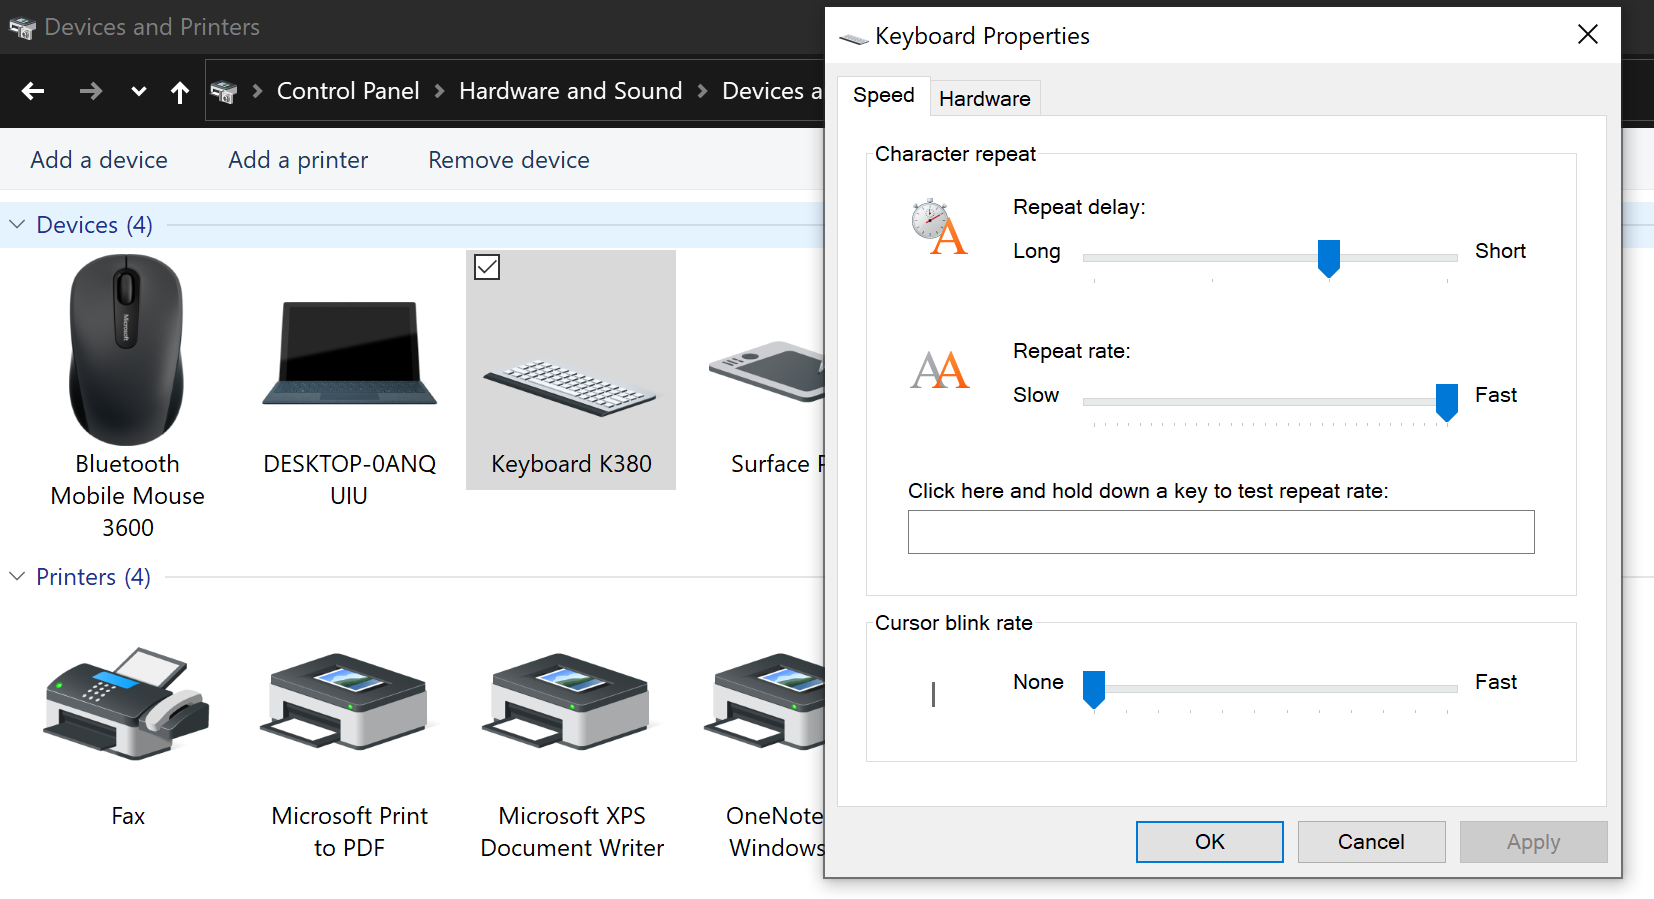
\includegraphics[width=.9\linewidth]{windows-setup/UnblinkCursor.PNG}
\end{center}
\end{document}
